\documentclass[10pt,a4j,twocolumn]{jsarticle}

\usepackage[dvipdfmx]{graphicx}
\usepackage{listings}
\setlength{\textheight}{275mm}
\headheight 5mm
\topmargin -30mm
\textwidth 185mm
\oddsidemargin -15mm
\evensidemargin -15mm
\pagestyle{empty}
\begin{document}
\title{ユーザメモソフトmy\_helpのビヘイビアテスト開発}
\author{関西学院大学 情報科学科 西谷研究室 2535 那須比呂貴}
\date{}
\maketitle
\section{目的}
プログラム開発では,統合開発環境がいくつも用意されているが,多くの現場では,terminal上での開発が一般的である.
ところが,プログラミング初心者はterminal上でのcharacter user interface(CUI)を苦手としている.
この不可欠なCUIスキルの習得を助けるソフトとして,ユーザメモソフトmy\_helpがruby gemsに置かれている.
しかし,Ruby gemsとして提供されているこのソフトは,動作はしますがテストが用意されていない.
今後ソフトを進化させるために共同開発を進めていくには,仕様や動作の標準となるテスト記述が不可欠である.
本研究の目的は,ユーザメモソフトであるmy\_helpのテストをBDDを用いて開発することである.

\section{先行研究,方法}
\subsection{BDDについて}
ビヘイビア駆動開発(Behaviour-Driven Development : BDD)は,テスト駆動開発(Test-Driven Development : TDD)の工程への理解を深め,それをうまく説明しようとして始まった.TDDの持つ単語のイメージが構造のテストを中心とするべしというのに対して,BDDはソフトの振る舞いに中心をおきなさいという意図がある.この違いが,初めに考えるべきテストの性質を変化させ,構造ではなく振る舞いを中心にテストを構築するという意識をもたせてくれる.
さらに,ソフトの中で,実世界において開発チームやテストチーム,あるいはドキュメントチーム間のコミュニケーションの取り方をシステムで提供しようというのがBDDのフレームワークであり,CucumberとRSpecはこれを実現する一つのシステムとして提供されている.
\subsection{CucumberとRSpecについて}
BDDの流れとして,まずCucumberで一つのシナリオに焦点を当てて,その振る舞いを記述するfeatureを書く.一つのfeatureが書けたら、次に,それぞれfeatureを実現するステップに分けて仕様を決めます.これはTDDのred green refactoringの前に行う作業,「仕様を決める」に対応していて.このプロセスが終了したら,RSpecに進む.
RSpecでは実際にテストコードを書き,ここでもred, green, refactoringをおこない,RSpecが成功したら,Cucumberのrefactoringをおこなう.
図1はRSpecとCucumberの関係図である.
\begin{figure}
\begin{center}
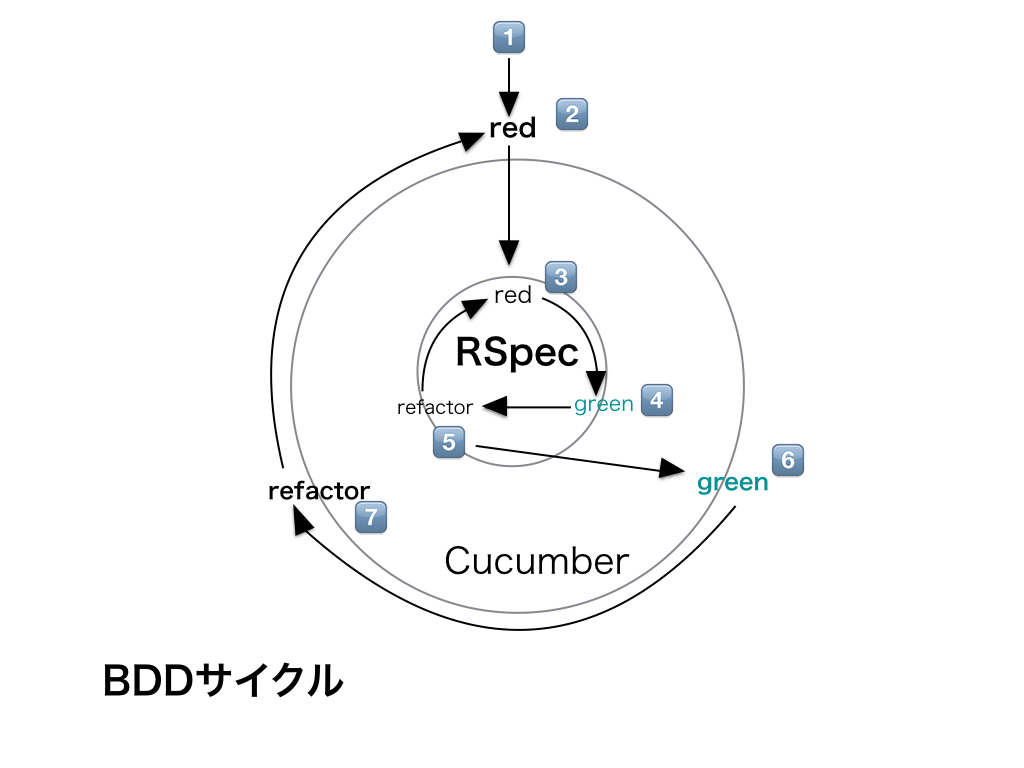
\includegraphics[width=8cm, bb=0 0 737 553]{my_help_nasu.001.png}
\caption{RSpecとCucumberのRed-Green-Refactoringサイクル間の関係.}
\end{center}
\vspace{0\baselineskip}
\end{figure}

また,Cucumberでは先ほど述べた通り、振る舞いをシナリオとしてまず記述する.
シナリオとは,一つひとつの振る舞いを,主にGiven(前提), Then(もし), When(ならば)に分けてfeaturesを記述する.
記述できたら,featureをcucumberコマンドで実行する.
実行するとステップ定義の元となるコードブロックが自動生成され,そこにあれば良いなと思うコードを記述していく.
ここまでが,cucumberの流れで,

\section{ビヘイビアテスト駆動開発の実践}
CucumberとRSpecを用いてBDDでmy\_helpのテスト開発を進めていった.
ここでは,焦点を合わせたmy\_helpの中での一つの振る舞いである「todoの更新」を例として詳しく見ていく.
まず,先に述べた通り「todoの更新」のシナリオをfeatureで記述する.
次にcucumberコマンドを実行し,ステップを記述する.
cucumberを実行するとステップの元なるコードブロックが自動生成されるので,それをコピーし,ペーストしてステップを
記述していく.
ここではあれば良いなと思うコードを記述し,もう一度cucumberを実行する.
あれば良いなと思うコードを記述しただけなので多分エラーが出るはずであり,そのエラーが出たシナリオに焦点をあて,RSpecに移行してテストコードを記述していく.
RSpecが成功したら,もう一度Cucumberに戻り,redをgreenにする.
このようにして,BDDを用いて,my\_helpの仕様や動作の標準を確定していった.

\section{研究の成果}
my\_helpのテスト記述が完了するに伴って,仕様や動作の標準が確定した.
my\_helpは今後も開発者,ならびに多くのユーザの使用を通じて,どのように進化させれば便利なのかが徐々にわかってくることで,my\_helpはまだまだ進化する機会が出てくると思われる.
つまり,ビヘイビアの記述を利用することで,今後my\_helpを進化させるための共同開発が円滑に進める手助けになると推測できる.
また,my\_helpの進化の開発だけに関わらず,my\_helpの使用方法が明確になったことで,本研究で作成したmy\_helpのfeaturesを読めば初心者でもmy\_helpの振る舞いが容易に理解できるようになった.
my\_helpは本研究室で今後使われていくと予想し,本研究はこれからの研究の手助けになる.

\section{今後の課題}
\begin{enumerate}
\item Cucumberを記述できるまで時間がかかる
\item BDDを行うときにrubyの知識が必要
\end{enumerate}

\begin{flushleft}
\begin{thebibliography}{99}
\bibitem{RSpecBook}   "The RSpec Book", David Chelimsky, Dave Astels, Zach Dennis, 訳, 株式会社クイーブ, 監修, 角谷信太郎, 豊田裕司 (翔泳社, 2012).
\bibitem{README}   my\_help README, Shigeot R. Nishitani, \verb|http://www.rubydoc.info/gems/my_help/0.4.3| 2017/2/11アクセス.
\bibitem{Qiita}   rake specにrspecのオプションを渡す, Qiita, \verb|http://qiita.com/snaka/items/e0808f9cfbad87c49b4e| 2017/2/13アクセス.
\end{thebibliography}
\end{flushleft}
\end{document}